%!TEX root = ../main.tex
\section{Advantages} % (fold)
\label{sec:advantages}

\subsection{Capturing a sinusoidal flow} % (fold)
\label{sub:capturing_a_sinusoidal_flow}

A sinusoidal function is injected in the convection toy problem:
\begin{equation}
	u_0(t) = \sin (2 \pi f_1 t) + \sin(2 \pi f_2 t).
\end{equation}
The signal is composed of two frequencies that will 
be chosen latter on.

\subsubsection{$f_1 = 1 \text{Hz}$, $f_2 = 0 \text{Hz}$}

This signal is made of a single frequency $f_1 = 1 \text{Hz}$.
The mono-frequential harmonic balance computation ran with only one harmonic
is shown Fig.~\ref{fig:convection_sin_1_tsm_n_1}.
\begin{figure}[htbp]
  \begin{center}
    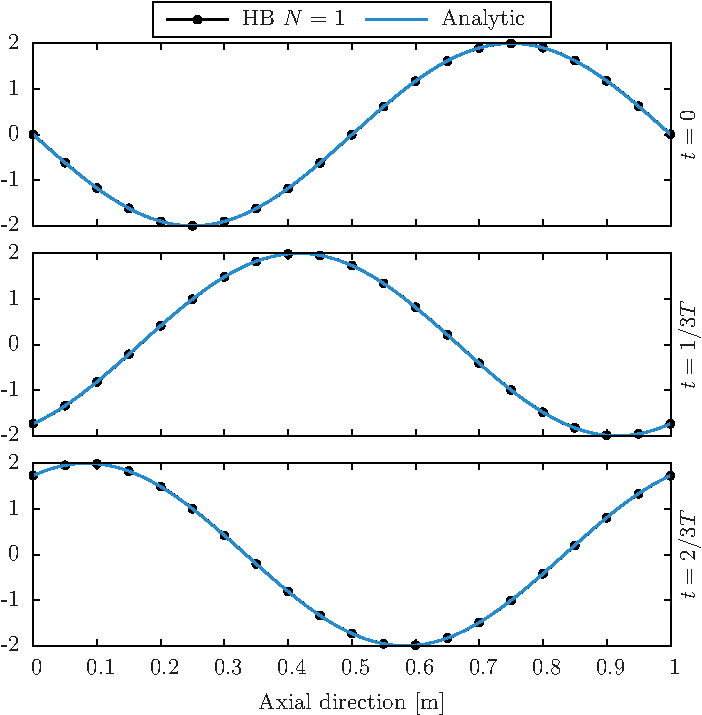
\includegraphics[width=.5\textwidth]{CONVECTION/FIGS/SIN_1/CONVECTION_SIN_1_TSM_N1.pdf}
  \end{center}
  \caption{Convection of a sinusoidal function.}
  \label{fig:convection_sin_1_tsm_n_1}
\end{figure}
The harmonic balance results match perfectly the analytical solution.
This was expected as harmonic balance methods have been developed to
easily capture periodic signals. When these are made of only one frequency,
one harmonic is sufficient to capture all the unsteadiness.

\subsubsection{$f_1 = 1 \text{Hz}$, $f_2 = 2 \text{Hz}$}



\subsubsection{$f_1 = 1 \text{Hz}$, $f_2 = 17 \text{Hz}$}

% subsection capturing_a_sinusoidal_flow (end)

% section advantages (end)